

Suppose $N\ge 1$ is an integer and define $h = 1/(N+1)$ and $x_j = ih$ for $i=0,\ldots, N+1$. We can approximate the differential equation
\[
-u''(x) = f(x), \quad 0<x<1,
\]
with homogeneous Dirichlet boundary conditions $u(0)=u(1) = 0$ by the matrix equation
\[
{-1 \over h^2} \left[\begin{array}{rrrrr}
              -2 & 1 \\[0.25em]
               1 & -2 & 1 \\
                 &  1  & -2 & \ddots \\
                 & & \ddots & \ddots & 1 \\[0.25em]
                 & & & 1 & -2 
               \end{array}\right]
          \left[\begin{array}{c} u_1 \\[0.25em] u_2 \\[0.25em] \vdots \\[0.25em] u_{N-1} \\[0.25em] u_N \end{array}\right]
 =   \left[\begin{array}{c} f(x_1) \\[0.25em] f(x_2) \\[0.25em] \vdots \\[0.25em] f(x_{N-1}) \\[0.25em] f(x_N) \end{array}\right],
\]
where $u_i \approx u(x_i)$.  (Entries of the matrix that are not specified are zero.)
\begin{enumerate}
\item Explain what adjustments to the right hand side of the matrix equation are necessary to accommodate the inhomogeneous Dirichlet boundary conditions
\[
u(0)=1,\quad  u(1)=2.
\]
\item Suppose that we have 
\begin{align*}
-u''(x) &= (2\pi)^2 \sin(2\pi x), \quad 0<x<1,\\
u(0) &= 1\\
u(1) &= 2.
\end{align*}
Since this differential equation is linear, we can split up the solution into 
$$u(x) = u_1(x) + u_2(x),$$ 
where $u_1(x)$ satisfies 
\begin{align*}
-u_1''(x) &= 0, \quad 0<x<1,\\
u_1(0) &= 1\\
u_1(1) &= 2
\end{align*}
and $u_2(x)$ satisfies the equation 
\begin{align*}
-u_2''(x) &= (2\pi)^2 \sin(2\pi x), \quad 0<x<1,\\
u_2(0) &= 0\\
u_2(1) &= 0.
\end{align*}
Show that $u(x) = u_1(x)+u_2(x)$ satisfies the original differential equation, and determine $u_1(x), u_2(x)$ and the exact solution $u(x)$.  %Hint: $u_1(x)$ is linear.
\item Compute and plot the approximate solutions for $N=8, 16, 32, 64$, and compare it to the exact solution $u(x)$.  On a separate plot, compute the maximum error $e_h$ for a given $h$
\[
e_{h} = \max_{0 \leq i \leq N+1} | u(x_i) - u_i |
\]
and plot $\log(h)$ against $\log(e_h)$ (in class, we showed this line should have slope $2$ - you may wish to check this is true by also plotting $\log(h)$ against $2\log(h)$ along with the error.  Both the error and this line should have identical slopes).  
\end{enumerate} 


%%%%%%%%%%%%%%%%%%%%%%%%%%%%%%%%%%%%%%%%%%%%%%%%%%%%%%%%%%%%

\ifthenelse{\boolean{showsols}}{

\begin{solution}

\begin{enumerate}
\item Since boundary conditions are applied at $u(x_0) = u_0$ and $u(x_{N+1}) = u_{N+1}$, they only show up in the finite difference equations for $x_1$ and $x_N$.  The finite difference equation at $x_1$ approximates $-u''(x_1) = f(x_1)$ via
\[
-\frac{u_2 - 2u_1 + u_0}{h^2} = f_1.
\]
Since $u_0 = u(x_0) = 1$ is known, we can modify the above equation to be
\[
-\frac{u_2 - 2u_1 }{h^2} = f_1 + \frac{1}{h^2}.
\]

Similarly, at $u_N = u(x_N)$, we approximate $-u''(x_N) = f(x_N)$ via
\[
-\frac{u_{N+1} - 2u_N + u_{N-1}}{h^2} = f_1.
\]
Since $u_{N+1} = u(x_{N+1}) = 2$ is known, we can modify the above equation to be
\[
-\frac{- 2u_N + u_{N-1}}{h^2} = f_1 + \frac{2}{h^2}.
\]
This leads to the system of equations
\[
{-1\over h^2} \left[\begin{array}{rrrrr}
              -2 & 1 \\[0.25em]
               1 & -2 & 1 \\
                 &  1  & -2 & \ddots \\
                 & & \ddots & \ddots & 1 \\[0.25em]
                 & & & 1 & -2 
               \end{array}\right]
          \left[\begin{array}{c} u_1 \\[0.25em] u_2 \\[0.25em] \vdots \\[0.25em] u_{N-1} \\[0.25em] u_N \end{array}\right]
 =   \left[\begin{array}{c} f_1  + \frac{1}{h^2}\\[0.25em] f_2 \\[0.25em] \vdots \\[0.25em] f_{N-1} \\[0.25em] f_N + \frac{2}{h^2} \end{array}\right],
\]
\item Since $-u_1''(x) = 0$, we know that $u_1$ should be a linear polynomial, or that 
\[
u_1(x) = ax + b.
\]
Boundary conditions then give 
\[
u(0) = 1 = b, \qquad u(1) = 2 = a + b
\]
or that $a = 1$, $b = 1$, and $u_1 = x + 1$. 

To solve $-u_2''(x) = (2\pi)^2\sin(2\pi x)$ with zero boundary conditions, we can note that $\sin(2\pi x)$ satisfies zero boundary conditions, and then observe that taking the negative of two derivatives of $\sin(2\pi x)$ gives back
\[
-\pd{\sin(2\pi x)}{x}{2} = (2\pi ^2)\sin(2\pi x).
\]
This implies that $u(x) = \sin(2\pi x)$ satisfies both the boundary conditions and the differential equation with inhomogenous source term.  
\item Included is Matlab code that can be used to generate the finite difference solution, exact solution, and the error between it and the exact solution.  

\emph{Graders: please do not take off if the students did not plot the error --- we only asked for a comparison of the exact solution to the computed solutions.}
\lstinputlisting{hw2_p2.m}
\begin{figure}
\centering
\subfigure[{Finite difference solutions for various $N$}]{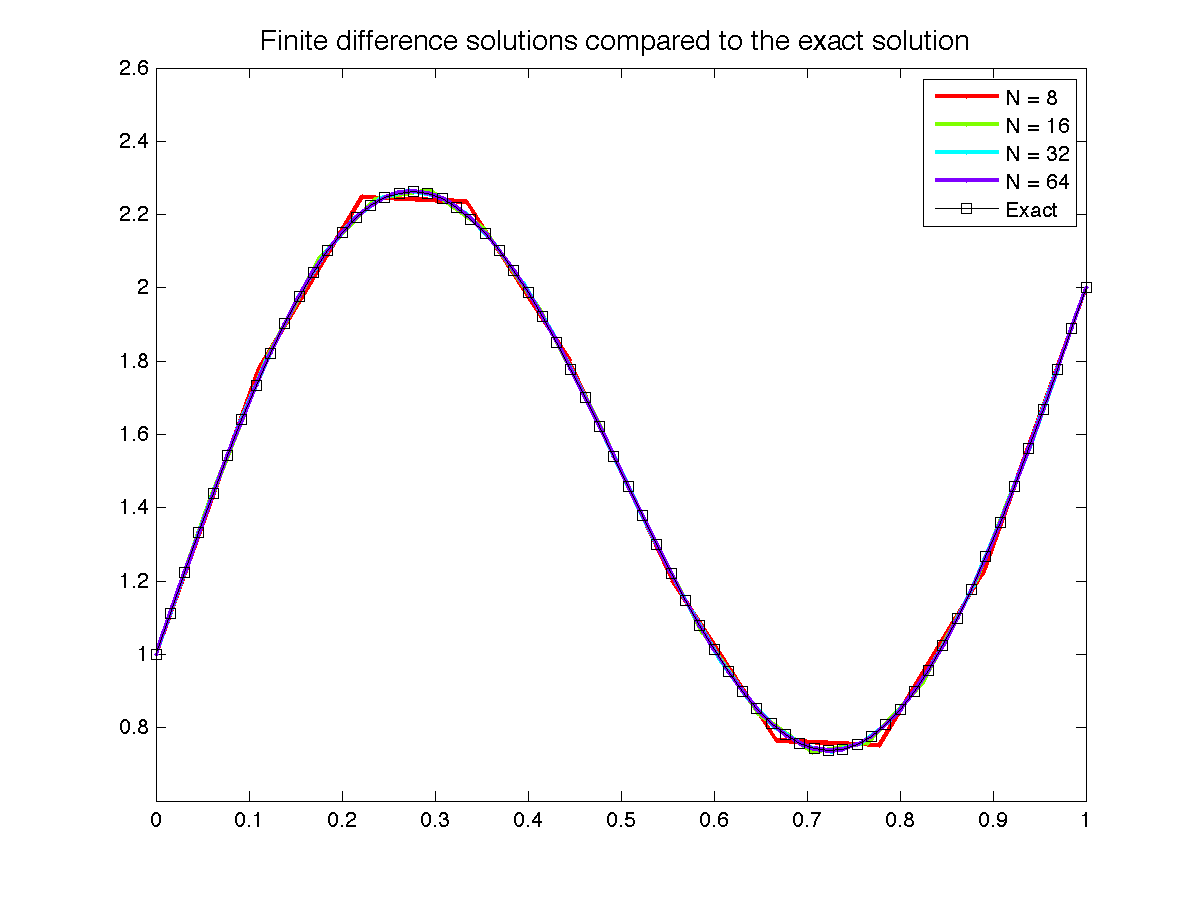
\includegraphics[width=.45\textwidth]{p2c_sol.png}}
\subfigure[Error between the exact solution and finite difference solution at points $x_i$.]{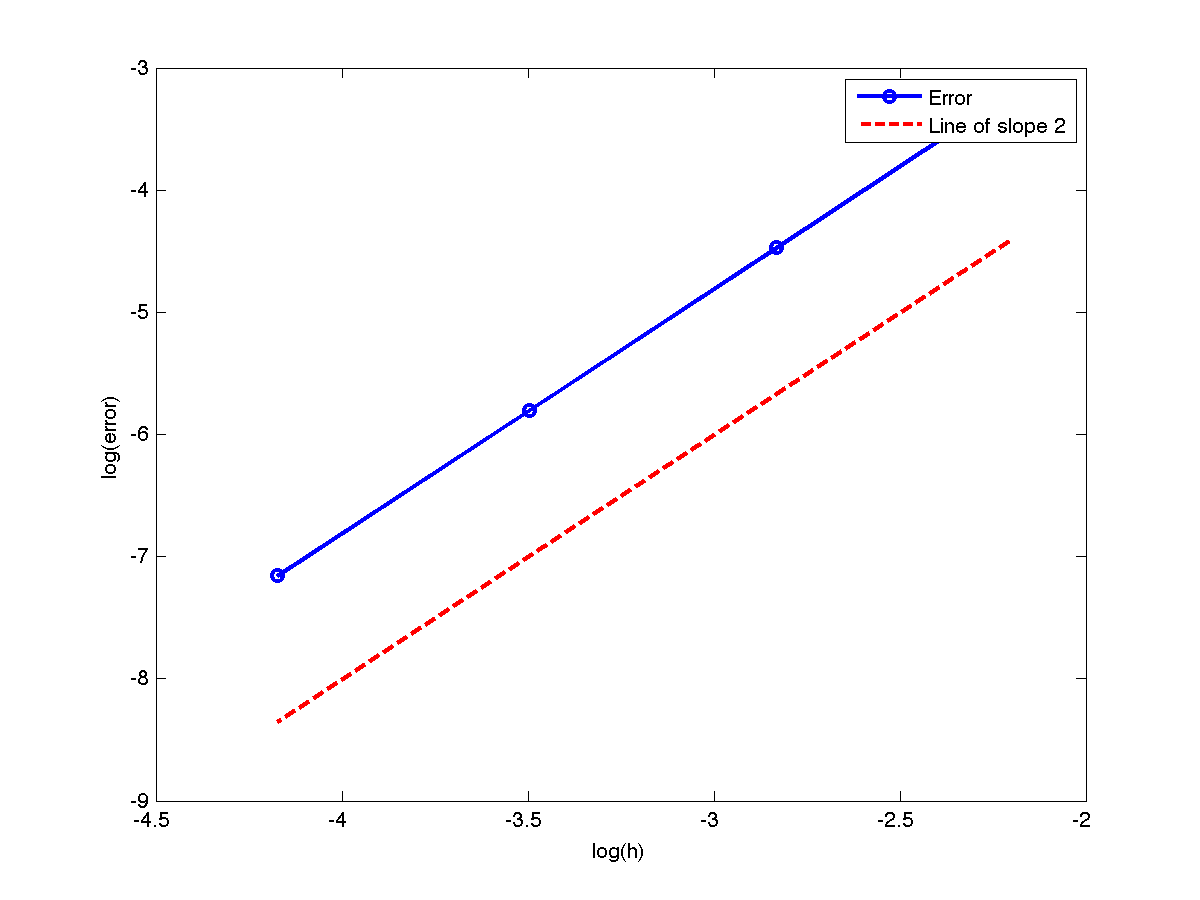
\includegraphics[width=.45\textwidth]{p2c_error.png}}
\end{figure}

\end{enumerate}  

\end{solution}
}

